\section{Lecture 22}
\subsection{Lecture Notes - Spinning Top with Torque, Nutation, Intro to Hamiltonian Mechanics}
\subsubsection{Returning to a Question}
We determined the scalar product $\v{L}^T\v{L}$ in the body frame. How does this compare to the scalar product in the space frame?
\begin{s}
The scalar product should be the same under rotation (invaraince under rotation). Going from the body frame to the space frame is just a rotation, and rotation preserves the angle between and the magnitude of two vectors. Another way to think about it:
\[\v{L}^T\v{L} = \v{L}'^TR^TR\v{L}' = \v{L}'^T\v{L}'\]
\end{s}
How does the rotational kinetic energy in the body frame $T = \frac{1}{2}\bm{\omega}^T\II\bm{\omega}$ compare to the rotational kinetic energy in the space frame.
\begin{s}
As above, the kinetic energy in the body frame and space frames should be equivalent. Mathematically:
\[\frac{1}{2}\bm{\omega}^T\II\bm{\omega} = \frac{1}{2}\bm{\omega}^{T'}RR^T\II RR^T\bm{\omega}' = \frac{1}{2}\bm{\omega}^{T'}\II\bm{\omega}'\]
\end{s}

\subsubsection{Spinning top with gravity/Nutation}
Last time, we derived an equation of motion for $\theta$ of a spinning top, and solved the equations for the case where $\theta$ was held constant. From this, we obtained the precession of the spinning top under gravity. We now consider the more general case where $\theta$ varies with time (is not constant). We will consider explicitly $\theta(t)$, and find "nutation"; that is, nodding repeatedly. Let us consider the energy:
\[E = T + U = \frac{\lambda_1}{2}\dot{\theta}^2 + U_{eff}(\theta)\]
Where:
\[U_{eff}(\theta) = \frac{(p_\phi - p_\psi\cos\theta)^2}{2\lambda_1\sin^2\theta} + \frac{p_\psi^2}{2\lambda_3} + MgR\cos\theta\]
(This was obtained just by replacing terms of $\dot{\phi}$ and $\dot{\psi}$ with the generalized momenta). This looks like the two body problem reduced to a one body problem with effective potential. We first notice that $MgR\cos\theta$ is negative for $\theta > \frac{\pi}{2}$ and $\frac{(p_\phi - p_\psi\cos\theta)^2}{2\lambda_1\sin^2\theta} + \frac{p_\psi^2}{2\lambda_3}$ is positive. At $\theta = 0, \pi$ we have that $U_{eff} \rightarrow \infty$. Graphically:
\begin{center}
    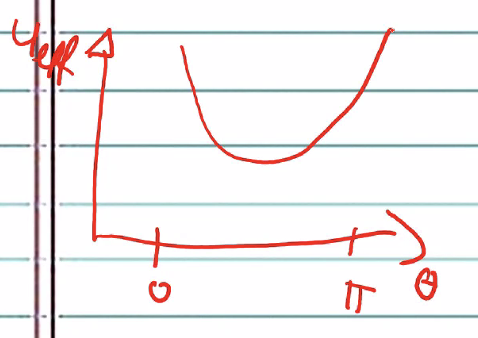
\includegraphics[scale=0.5]{Lecture-22/l22-img1.png}
\end{center}
Now consider:
\begin{center}
    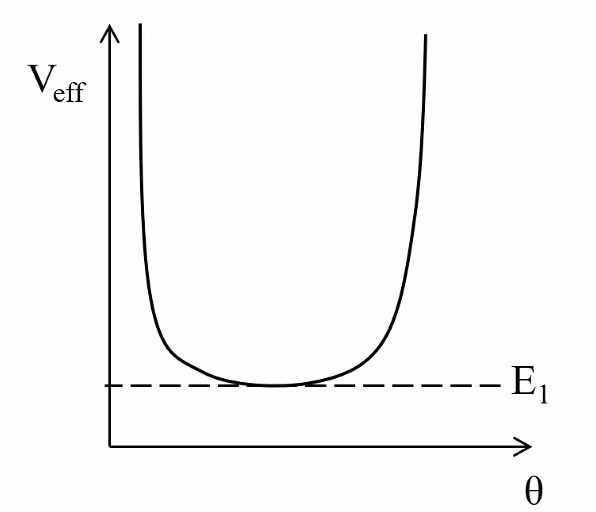
\includegraphics[scale=0.5]{Lecture-22/l22-img2.png}
\end{center}
If a symmetric top has total effective energy $E_1$, then what type of motion does this top undergo?
\begin{s}
The top undergoes constant precession about the vertical axis, at a constant $\theta$; we have not excited the one dimensional system, and $\theta$ must hence be constant (stay in the minimum)
\end{s}
If we now give it some energy:
\begin{center}
    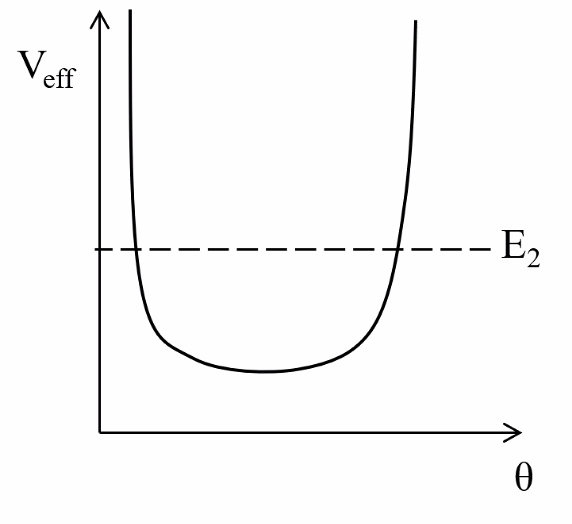
\includegraphics[scale=0.5]{Lecture-22/l22-img3.png}
\end{center}
What is the motion?
\begin{s}
The top will now undergo precession combined with nutation, as $\theta$ oscillates about the minimum. 
\end{s}
There are several qualitatively different scenarios that can occur. We have the equation:
\[\dot{\phi} = \frac{p_\phi - p_\psi\cos\theta}{\lambda_1\sin^2\theta}\]
Two possible scenarios are:
\begin{center}
    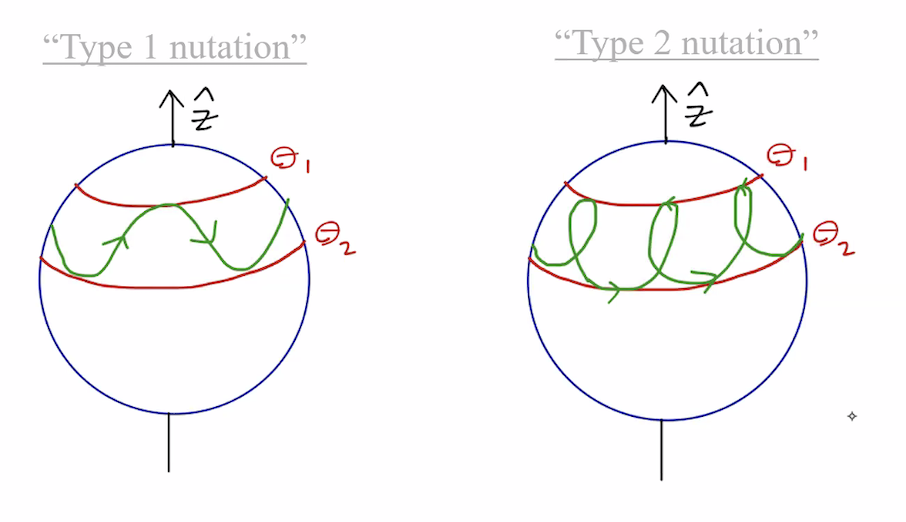
\includegraphics[scale=1]{Lecture-22/l22-img4.png}
\end{center}
The first scenario occurs where $p_\phi > p_\psi$ and $\dot{\phi} > 0$. The second scenario occurs where $p_\phi \approx p_\psi$, then we have $p_\phi < p_\psi\cos\theta$ and $p_\phi > p_\psi\cos\theta_2$ and hence we have that $\dot{\phi}$ changes direction (which is quite cool!) There is also a third case, where we get cusps:
\begin{center}
    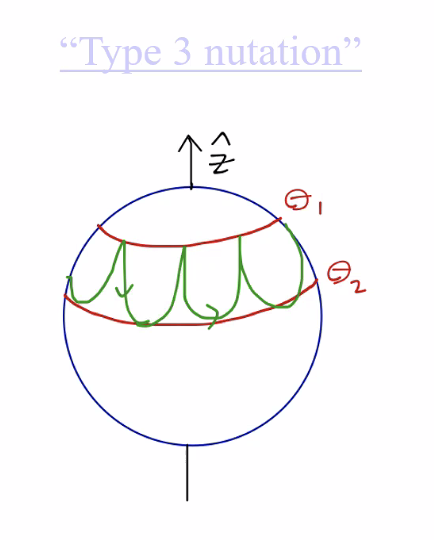
\includegraphics[scale=0.8]{Lecture-22/l22-img5.png}
\end{center}
Where $p_\phi \approx p_\psi$ and we can have $p_\phi = p_\psi\cos\theta_1$ or $p_\phi = p_\psi\cos\theta_2$.

\subsubsection{Intro to Hamiltonian Mechanics - Motivation}
Why do we need another form of mechanics? Newton was nice and intuitive, and Lagrange is much easier if we have constraints in our system and want to solve problems without having to explicitly worry about the constraints. Why can't we just be happy with Lagrange and leave it as it is? Reason 1 is that its cool/beautiful. From a practical perspective, it doesn't give us much of an advantage over Lagrange, but it will allow us to give a richer understanding of dynamical systems and conserved quantities. There is also an advantage when we want to link this to the most important theory of 20th century physics, that is, quantum mechanics. 

\subsubsection{What was the Hamiltonian, Again?}
As a reminder, we have the Lagrangian:
\[\LL = \LL(q_1, q_2, \ldots, q_n, \dot{q}_1, \dot{q}_2, \cdots, \dot{q}_n)\]
We also introduced the generalized, or canonical momentum:
\[p_i = \dpd{\LL}{\dot{q}_i}\]
We then defined the Hamiltonian:
\[\HH = \sum_{i=1}^mp_i\dot{q}_i - \LL\]
When the transformation from cartesian to generalized coordinates was natural (did not depend on time), then $\HH$ was just the total energy. For further applications in this course, we will generally assume this is the case. The Hamiltonian is a function:
\[\HH = \HH(q_1, q_2, \ldots, q_n, \dot{q}_1, \dot{q}_2, \cdots, \dot{q}_n, t)\]
The main difference is that we trade between the generalized velocities (Lagrangian) with the generalized momentum (Hamiltonian). How does this occur? We will see in a moment, but let us do a basic example first. 

\subsubsection{The Harmonic Oscillator}
The Lagrangian for the Harmonic oscillator is:
\[\LL = \frac{m}{2}\dot{x}^2 - k\frac{x^2}{2}\]
So the generalized momentum is:
\[\dpd{\LL}{\dot{x}} = m\dot{x} = p\]
So calculating $\HH$, we have:
\[\HH = m\dot{x}^2 - \LL = \frac{m}{2}\dot{x}^2 + k\frac{x^2}{2} = \frac{p^2}{2m} + k\frac{x^2}{2} =  T + U\]
Calculating $\HH$ is pretty straightforward.

\subsubsection{The Hamiltonian as the Legendre Transform of L}
Consider a function $f(x,y)$. The total differential is then given by:
\[df = \dpd{f}{x}dx + \dpd{f}{y}dy  = udx + vdy\]
Now, we want to "trade" the differentials, $x \mapsto u$. We can do this via a function $g = f - ux$. Let's check:
\[dg = df - udx - xdu\]
But we've already calculated $df$, so:
\[df = udx + vdy - udx - xdu = vdy - xdu\]
So as advertised, $g$ is the Legendre transform of $f$, and it depends explictly on the variables $u$ and $y$:
\[g = g(u, y)\]
To recap, we look at the total differential, we want to trade one function against the other, we then construct a function such that the independent variables are swapped. This has connections to thermodynamics; we recall that the energy of a thermodynamic system is dependent on the natural variables of number of particles, volume, and entropy, that is $E = E(N, V, S)$. But we had other relevant quantities, such as the Hemholtz free energy; $F = E - TS = F(N, V, T)$. Hence, the varaibles $S$ and $T$ are conjugate to each other. In many cases, its more convenient to use $F$ as it is easier to control the temperature rather than the entropy. In classical mechanics, it might be more convenient to work with the momenta rather than velocities, and easier to work with $\HH$ rather than $\LL$. 

\subsubsection{Hamilton Equations of Motion}
We need to see what kind of equations of motion come out of this formulation of classical mechanics. Let's write the hamiltonian as:
\[\HH = \sum_i p_i\dot{q}_i - \LL\]
Now, consider the total differential of $\HH$. We have:
\[d\HH = \sum_i \left(\dot{q}_i dp_i + p_i d\dot{q}_i\right) - \dpd{\LL}{q_i}dq_i - \dpd{\LL}{\dot{q}_i}d\dot{q}_i - \dpd{\LL}{t}dt\]
If we recall the definitions, the $\dpd{\LL}{\dot{q}_i}$ term is just $p_i$, and $\dpd{\LL}{q_i}$ is just $\dot{p}_i$ if we use the Euler-Lagrange equation. Hence the above becomes:
\[d\HH = \sum_i (-\dot{p}_idq_i + \dot{q}_idp_i) - \dpd{\LL}{t}dt\]
Hence we can read off the differential:
\[\boxed{\dpd{\HH}{p_i} = \dot{q}_i, \dpd{\HH}{q_i} = -\dot{p}_i}\]
And these are Hamilton's equations! We will look at these more closely on Friday.